\documentclass{beamer}
\usepackage{array}
\usepackage{graphicx}
\usetheme{Madrid}

% Suppress the navigation bar and remove name and date from slides
\setbeamertemplate{navigation symbols}{}
\setbeamertemplate{footline}{}  % Removes the footer line with the author and date
\setbeamertemplate{headline}{}  % Removes the header line

% Title page details
\title{Conversational Used Car Price Predictor}
\subtitle{CS702 - Computing Lab}
\author{ABHIJITH C \and ANAND M K}
\institute{Department of Computer Science and Engineering \\ NITK Surathkal}
\date{}  % No date on title slide

\begin{document}

% Title page
\begin{frame}[t]
    \titlepage
\end{frame}

% Slide 1: Introduction
\begin{frame}[t]{Introduction}
    \begin{columns}
        \column{0.6\textwidth}
        \begin{itemize}
            \item Conversational interfaces enhance interaction with technology.
	\item With the advancements in Natural Language Processing (NLP) and conversational interfaces, chatbots have become an effective way to improve user experience and interaction by providing a more natural, engaging, and flexible platform.
            \item By integrating a chatbot into a used car price prediction system, users can interact in a more conversational way
        \end{itemize}
        
        \column{0.4\textwidth}
        \centering
        
\includegraphics[width=\linewidth]{Chatbot.jpg}  % Replace 'your_image.png' with your image file
    \end{columns}
\end{frame}

% Slide 2: Problem Statement and Objectives
\begin{frame}[t]{Problem Statement and Objectives}
    \begin{columns}
        \column{0.6\textwidth}
        \begin{itemize}
        \item Predicting used car prices requires multiple parameters such as manufacturer, model, year, mileage, etc.
        \item Traditional methods require users to interact with a web form or mobile app input fields to submit the necessary car details,which are often less interactive and user-friendly.
        \item This project aims to develop a chatbot integrated with a price prediction model for a more intuitive user experience.
        \end{itemize}
        
        \column{0.4\textwidth}
        \centering
        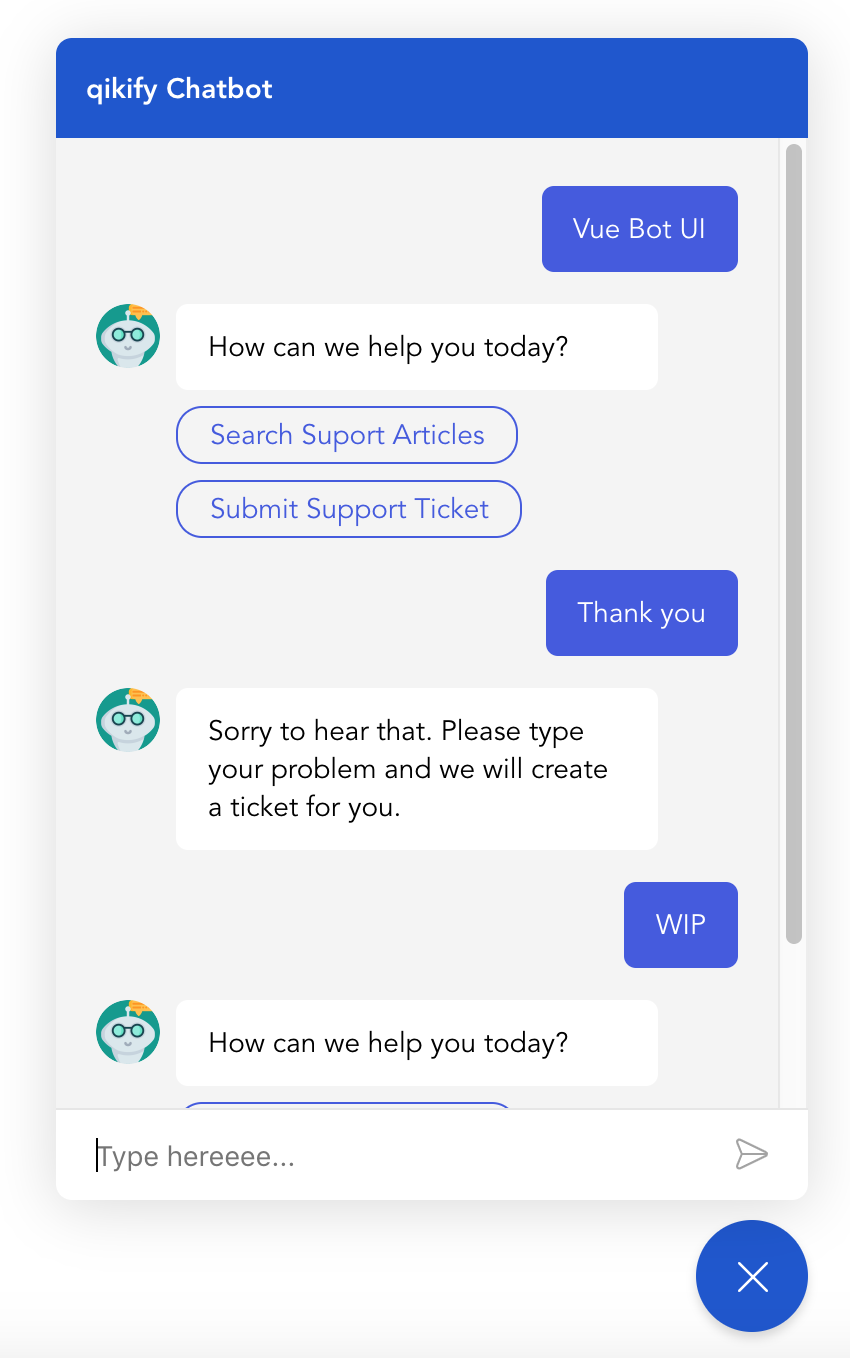
\includegraphics[width=\linewidth]{interface.png}  % Replace 'your_image.png' with your image file
    \end{columns}
\end{frame}

% Slide: Literature Survey with Table
\begin{frame}[t]{Literature Survey}
    \footnotesize % Further reduce font size for table content
    \resizebox{\textwidth}{!}{  % Rescale the table to fit the slide
    \begin{tabular}{|c|m{4cm}|c|m{5cm}|}
        \hline
        \textbf{S.No.} & \textbf{Title} & \textbf{Year} & \textbf{Methodology} \\ \hline
        1 & Prediction of Used Car Prices Using Artificial Neural Networks and Machine Learning & 2022 & Deep Neural Networks, Linear Regression, Random Forest Algorithm \\ \hline
        2 & Predicting the Sale Price of Pre-Owned Vehicles with the Ensemble ML Model & 2023 & Linear Regression Model, Random Forest Regression, Gradient Boosting Tree (GBT) Regression Model \\ \hline
        3 & An Overview of Chatbot Technology & 2020 & Rule-Based Model Chatbots, Generative Models. Development platforms can be open-source, such as RASA. \\ \hline
        4 & Conversational AI Unleashed: A Comprehensive Review of NLP-Powered Chatbot Platforms & 2023 & Rule-Based Systems, Generative Models. \\ \hline
        5 & Framework for Design and Implementation of Chat Support System using Natural Language Processing & 2023 & The chatbot is developed in Django web framework and spaCy NLP library for Python. \\ \hline
    \end{tabular}
    }
\end{frame}



\begin{frame}[t]{Proposed Methodology}
        \centering
        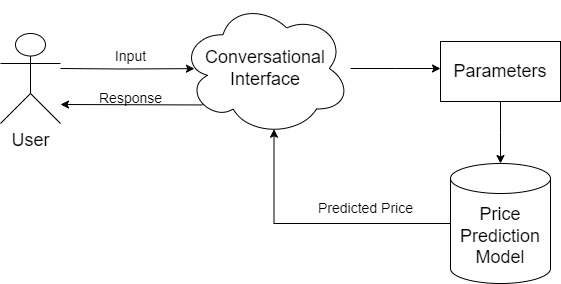
\includegraphics[width=0.7\linewidth]{Proposed.png}  % Replace 'your_image.png' with your image file
    \begin{itemize}
            \item Conversational Interface: The proposed system will integrate a chatbot that will act as the primary interface for user interaction. Instead of filling out forms, users will engage in a natural language conversation to provide the necessary details about their car.
	 \item Guided Data Collection: The chatbot will guide users step by step, asking questions about the car’s make, model, year, mileage, condition, and other relevant factors in a user-friendly, conversational manner.


    \end{itemize}
\end{frame}

\begin{frame}[t]{Finalized Design of Solution}
    \begin{itemize}
        \item \textbf{System Architecture:}
	\begin{figure}[htbp]
        \centering
        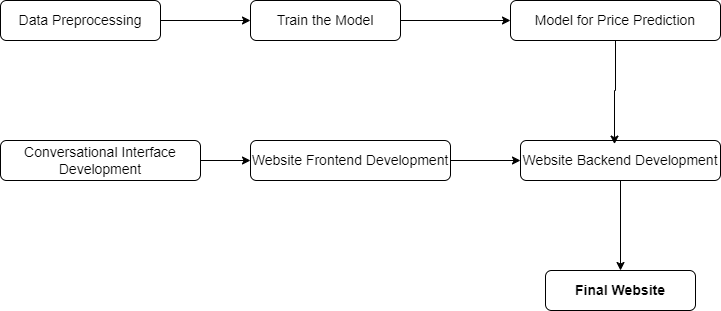
\includegraphics[width=0.8\textwidth]{Flowchart2.png}
    \end{figure}
        \begin{itemize}
            \item \textbf{NLP Engine:} Processes natural language inputs, extracts intents and entities, and manages conversation flow.
            \item \textbf{Prediction Model:} A machine learning model that predicts the price of the car based on the extracted data from user inputs.
            \item \textbf{Frontend:} A website providing a chat interface for users to interact with the system.
            \item \textbf{Backend:} A server that processes user inputs, communicates with the NLP engine and the prediction model, and handles responses.

        \end{itemize}
    \end{itemize}

	
\end{frame}

\begin{frame}[t]{Experimental Setup}
    \begin{itemize}
        \item Frontend: HTML, CSS, JavaScript for creating a responsive chat interface.
        \item Backend: Python framework (Flask or Django) to handle interactions between the frontend, Rasa NLP engine, and the prediction model.
        \item NLP Engine: Rasa will be used to implement a rule-based chatbot. It will process natural language inputs to extract intents and entities, and trigger predefined actions.
        \begin{itemize}
            \item \textbf{Intents:} User intents include providing car details, requesting price prediction, and asking for help or guidance.
            \item \textbf{Entities:} The chatbot will extract entities such as car make, model, year, mileage, and kilometers driven from the conversation.
            \item \textbf{Actions:} Actions include validating user input, passing car details to the prediction model, and returning the predicted price.
        \end{itemize}
        \item Prediction Model: Machine learning model (random forest or any other regression model) for predicting used car prices based on user inputs.
        \item Dataset: The dataset for training the prediction model will be sourced from Kaggle.
    \end{itemize}
\end{frame}

\begin{frame}[t]{Expected Outcomes}
    \begin{itemize}
        \item A user-friendly conversational interface that will guide users through the process of providing necessary car details in a natural and interactive manner.
        \item Successful integration of the Rasa rule-based chatbot for handling user inputs, understanding intents, and extracting entities such as car make, model, year, and mileage.
        \item An accurate machine learning model capable of predicting used car prices based on the extracted details.
        \item Seamless communication between the frontend, backend, and prediction model to provide real-time price estimates to users.
    \end{itemize}
\end{frame}

\begin{frame}[t]{Conclusion and Future Work}
    \begin{itemize}
        \item This project successfully integrates a conversational interface with a used car price prediction model, making the user experience more interactive and efficient.
        \item \textbf{Future Work:}
        \begin{itemize}
            \item Introduce voice command functionality for hands-free user interaction.
            \item Add support for multiple languages using translation functionality. 
        \end{itemize}
    \end{itemize}
\end{frame}

\begin{frame}[t]{References}
\begin{thebibliography}{9}
\bibitem{varshitha2022}
J. Varshitha, K. Jahnavi, and C. Lakshmi, "Prediction Of Used Car Prices Using Artificial Neural Networks And Machine Learning," \textit{2022 International Conference on Computer Communication and Informatics (ICCCI)}, Coimbatore, India, 2022, pp. 1-4, doi: 10.1109/ICCCI54379.2022.9740817.

\bibitem{kathiravan2023}
M. Kathiravan, M. Ramya, S. Jayanthi, V. V. Reddy, L. Ponguru, and N. Bharathiraja, "Predicting the Sale Price of Pre-Owned Vehicles with the Ensemble ML Model," \textit{2023 4th International Conference on Electronics and Sustainable Communication Systems (ICESC)}, Coimbatore, India, 2023, pp. 1793-1797, doi: 10.1109/ICESC57686.2023.10192988.

\bibitem{kathiravan2021}
Shubham Chaurasia , Shubha Jain , Hari Om Vishwkarma , Nishant Singh "Conversational AI Unleashed: A Comprehensive Review of NLP-Powered Chatbot Platforms" Iconic Research And Engineering Journals Volume 7 Issue 3 2023 Page 1-8


\end{thebibliography}
\end{frame}

\begin{frame}[t]{References}
\begin{thebibliography}{9}
\bibitem{kathiravan2019}
P. William, G. R. Lanke, V. N. R. Inukollu, P. Singh, A. Shrivastava and R. Kumar, "Framework for Design and Implementation of Chat Support System using Natural Language Processing," 2023 4th International Conference on Intelligent Engineering and Management (ICIEM), London, United Kingdom, 2023, pp. 1-7, doi: 10.1109/ICIEM59379.2023.10166939. keywords: {Costs;Customer services;Power distribution;Companies;Chatbots;Libraries;Task analysis;Chatbot;Natural Language Processing;Django;spaCy;Chatbot based Customer Support},

\bibitem{kathiravan2018}
Adamopoulou, E., Moussiades, L. (2020). An Overview of Chatbot Technology. In: Maglogiannis, I., Iliadis, L., Pimenidis, E. (eds) Artificial Intelligence Applications and Innovations. AIAI 2020. IFIP Advances in Information and Communication Technology, vol 584. Springer, Cham. 

\end{thebibliography}
\end{frame}

\begin{frame}[t]{.}
    \centering
    \vspace{1cm}
    \textbf{\Huge{}}
    
    \vspace{0.5cm}
    \rule{0.5\textwidth}{0.5mm} % Horizontal line for design

    \vspace{1cm}
    \textbf{\Large{Thank You!}}

    \vspace{0.5cm}
    \rule{0.5\textwidth}{0.5mm} % Another horizontal line for symmetry
\end{frame}


\end{document}
